\section{El Niño DDE}
\rhead{El Niño DDE}


\subsection{Gleichung}
Zur Modellierung des El Niño Effektes wurde im Kapitel \ref{section:dde-nino} die folgende DDE gefunden
\begin{equation} \label{eldde}
\dot{T}(t)=-cT(t)+aT(t-\frac{1}{2}\tau_K)-bT(t-(\frac{1}{2}\tau_R+\tau_K)).
\end{equation}
Mit dieser DDE wird die Änderung der Meerestemperaturanomalie $T$ vor der Küste Südamerikas beschrieben.
Die Konstanten $c,a,b$ müssen so bestimmt werden, dass die DDE ein möglichst gutes Resultat ergibt.
Erst wenn diese Konstanten grob bestimmt sind, kann eine sinnvolle numerische Simulation gestartet werden.
Hilfreich sind vor allem ungefähre Verhältnisse zwischen den Konstanten, so dass man zumindest einen Anhaltspunkt für die Simulation hat.
Die Verzögerungen $\tau_K$ und $\tau_R$ sind ungefähr bekannt aus physikalischen Untersuchungen der Rossby- und Kelvinwellen (vgl. \cite[Kaper]{verzoegert:kaperengler}).
\begin{equation}
	\tau_K \approx \frac{1}{6}yr \text{ und } \tau_R \approx 1 yr
\end{equation}


\subsection{Charakteristische Gleichung}
Die charakteristische Gleichung für die DDE \eqref{eldde} scheint schwierig zu sein. 
Aus diesem Grund vereinfachen wir die DDE so weit, bis wir einen Ansatz versuchen können.
Weil $\tau_K \ll \tau_R$ setzen wir $\tau_K = 0$ und erhalten
\begin{equation}
	\dot{T}(t)=-cT(t)+aT(t)-bT(t-(\frac{1}{2}\tau_R)).
\end{equation}
Nun stellen wir eine einfache DDE auf, mit $\alpha = a-c$, $\beta = b$ und $\tau = \frac{1}{2}\tau_R$.
\begin{equation}
	\dot{T}(t)=\alpha T(t)-\beta T(t-\tau)
\end{equation}
In diese DDE setzen wir nun den bekannten Ansatz $e^{\lambda t}$ mit $\lambda \in \mathbb{C}$ ein und erhalten
\begin{equation} \label{char_eldde}
	\lambda e^{\lambda t} = \alpha e^{\lambda t} - \beta e^{\lambda(t-\tau)} \qquad\Rightarrow\qquad \lambda = \alpha-\beta e^{-\lambda \tau}.
\end{equation}
Es sind beliebig viele Lösungen für $\lambda$ und die Konstanten möglich.
Wir suchen nun die Lösung, welche dem El Niño Phänomen entspricht.
Da der El Niño in grober Näherung ohne Dämpfung oszilliert (vgl. Abbildung \ref{fig:elnino}), betrachten wir nur die Lösungen bei denen $\lambda$ rein imaginär wird.
\begin{figure}
	\centering
	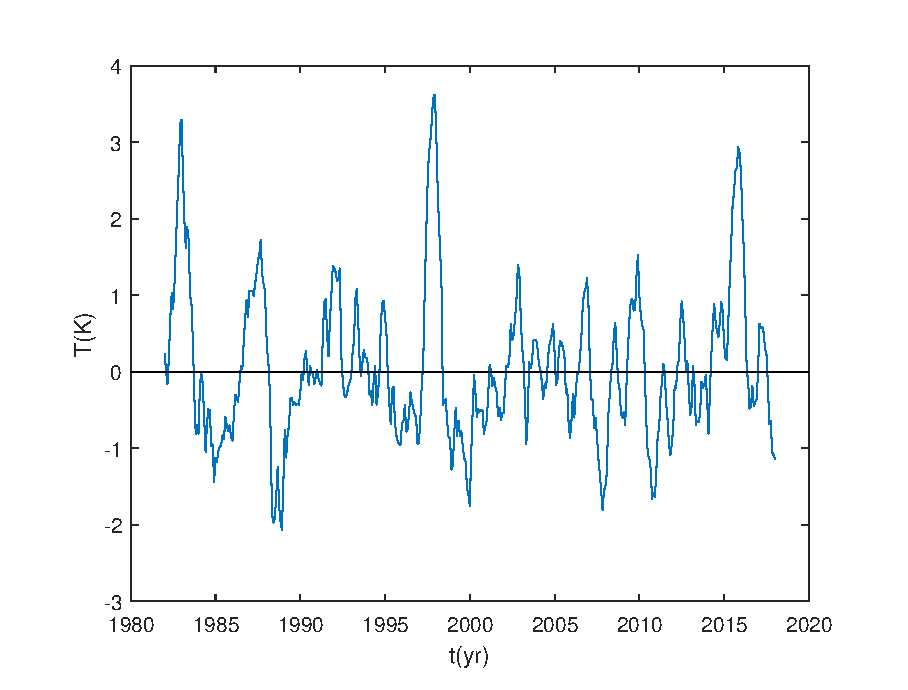
\includegraphics{verzoegert/inp/figures/elnino.eps}
	\caption{El-Niño (Temperaturanomalie $T$ vor der Küste Südamerikas) gemessen von 1982 bis 2017}
	\label{fig:elnino}
\end{figure}
Wir setzen also $\lambda = i\omega$ und nach der Formel von Euler wird die Gleichung \eqref{char_eldde} umgeschrieben zu 
\begin{equation}
	 i\omega = \alpha-\beta(\cos(-\omega \tau)+i\sin(-\omega \tau)).
\end{equation}
Es ergeben sich daraus zwei Gleichungen für Imaginär- und Realteil
\begin{equation} \label{bed1}
  	\alpha-\beta\cos(\omega \tau) = 0 \quad\text{und}\quad \beta\sin(\omega\tau)=\omega.
\end{equation}
Wenn diese beiden Gleichungen miteinander dividiert werden, erhalten wir die Bedingung
\begin{equation} \label{bed}
	\tan(\omega\tau)=\frac{\omega}{\alpha}.
\end{equation}
 
\subsection{Berechnen der Konstanten}
Aus der Bedingung \eqref{bed} können die Konstanten näherungsweise berechnet werden.
Zuerst geben wir die Kreisfrequenz der Oszillation $\omega$ an. 
Auf der Abbildung \ref{fig:elnino} können wir mit etwas Phantasie eine Periodendauer zwischen drei und sieben Jahren erkennen.
Wir bestimmen für die folgenden Berechnungen eine durchschnittliche Periodendauer von 4 Jahren. 
Eine plausible Periode könnte mit Hilfe der Fouriertheorie (vgl. Kapitel \ref{chapter:fourier}) bestimmt werden.
Alle Zeitangaben werden in Jahren angegeben.

Aus der Periodendauer ergibt sich $\omega = \frac{2\pi}{T_\text{Periode}} = \frac{\pi}{2}$ und aus der Bedingung \eqref{bed} erhalten wir nun 
\begin{equation}
	a-c=\alpha=\frac{\omega}{\tan(\frac{1}{2}\tau_R \omega)}=\frac{\frac{\pi}{2}}{\tan(\frac{\pi}{4})}=\frac{\pi}{2}\approx 1.6.
\end{equation}
Weiter berechnen wir $\beta$ aus \eqref{bed1} und erhalten
\begin{equation}
	b=\beta=\frac{\omega}{\sin(\frac{1}{2}\tau_R \omega)}=\frac{\frac{\pi}{2}}{\sin(\frac{\pi}{4})}\approx 2.3.
\end{equation}

\subsection{Chaotisches Verhalten}
Die Lösungen der Gleichung \eqref{eldde} zeigen ein chaotisches Verhalten.
Chaotisches Verhalten bedeutet, dass kleinste Änderungen der Konstanten extrem unterschiedliche Lösungen verursachen können. 
\begin{figure}
	\centering
	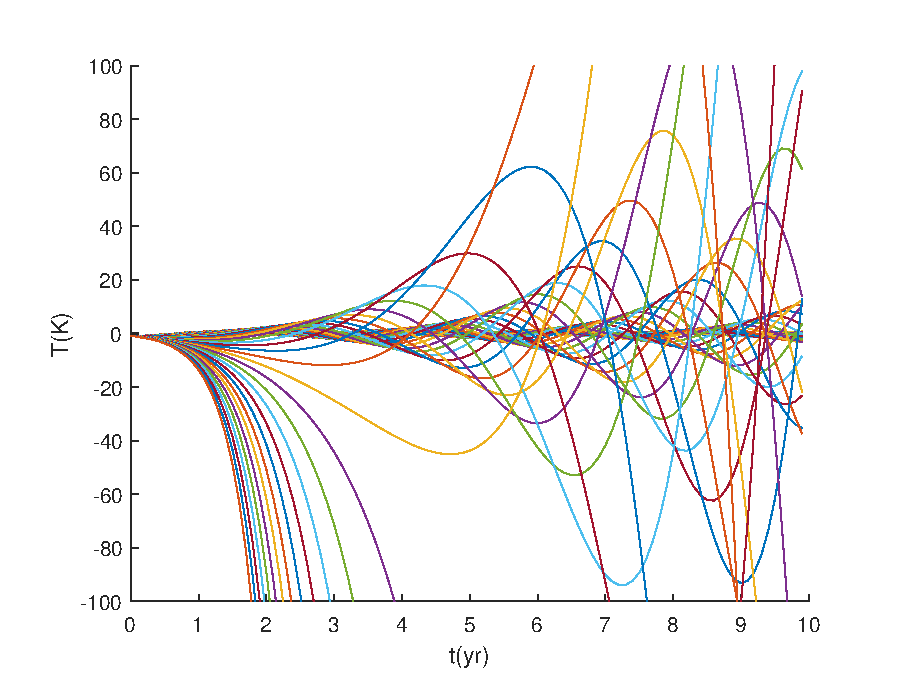
\includegraphics{verzoegert/inp/figures/param_a_e0.eps}
	\caption{Chaotisches Verhalten bei der Änderung von $a=0$ bis $a=5$}
	\label{fig:chaos}
\end{figure}
In Abbildung \ref{fig:chaos} sieht man das chaotische Verhalten bei einer Änderung der Konstante $a$.
Dieses Verhalten ist unerwünscht, da wir die Ausgangslage nicht genau kennen und die Konstanten anpassen müssen.
Um dieses chaotische Verhalten zu unterbinden, wird ein Limitierungsterm eingeführt.
Dieser besteht aus $-\varepsilon T(t)^3$ und verhindert explodierende Lösungen.
Bei zunehmendem Funktionswert nimmt der limitierungsterm mit der dritten Potenz zu und dämpft somit den Funktionswert.
Wir erhalten die Gleichung
\begin{equation} \label{eldde_epsilon}
\dot{T}(t)=-cT(t)+aT(t-\frac{1}{2}\tau_K)-bT(t-(\frac{1}{2}\tau_R+\tau_K))-\varepsilon T(t)^3.
\end{equation}
In Abbildung \ref{fig:chaos_fix} wird die gleiche Änderung von $a$ gezeigt, aber mit einem $\varepsilon = 0.1$.
Man sieht nun sehr gut den Einfluss, den die Konstante $a$ auf die Lösung hat (verändert Frequenz und Amplitude).
\begin{figure}
	\centering
	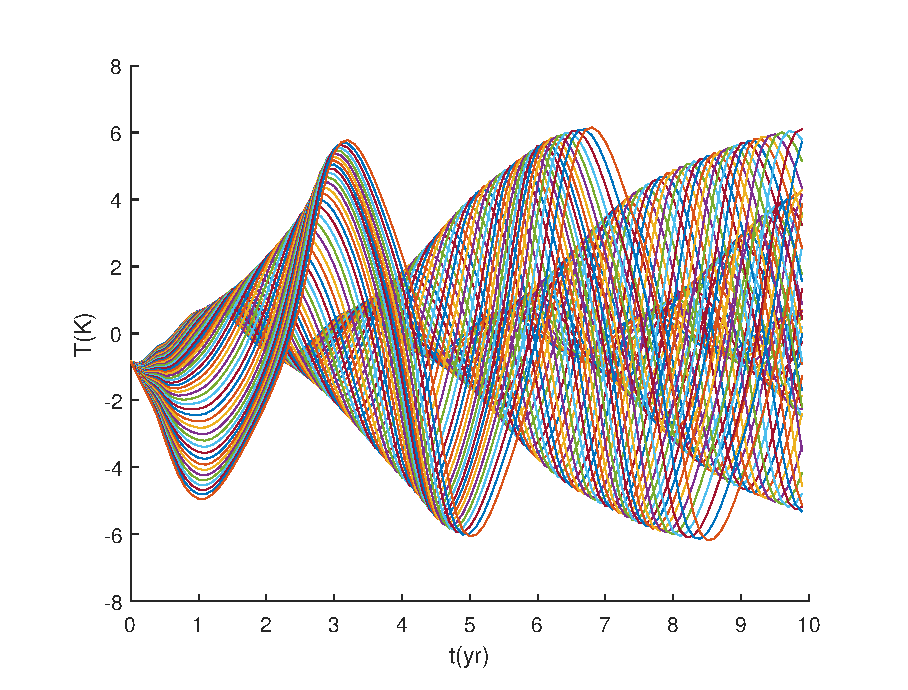
\includegraphics{verzoegert/inp/figures/param_a_e01.eps}
	\caption{Verhalten bei der Änderung von $a=0$ bis $a=5$ mit Limitierung $\varepsilon = 0.1$}
	\label{fig:chaos_fix}
\end{figure}
